\documentclass[letterpaper,10pt,conference]{IEEEtran}

\usepackage{amsmath,amssymb}
\usepackage{booktabs}
\usepackage{balance}
\usepackage{graphicx}
\usepackage{url}
\usepackage{xcolor}

\graphicspath{{figures/}}
\newcommand{\R}{\mathbb{R}}
\newcommand{\T}{\mathsf{T}}

\title{Lab 2: Rigid-Body Transformations and Relative Trajectories in ROS}

\author{\IEEEauthorblockN{Student Name \quad Student ID}
\IEEEauthorblockA{Integrated Project\\
Institution Name\\
Email: student@example.com}}

\begin{document}
\maketitle

\begin{abstract}
The MIT VNAV Lab 2 two-drone scenario is implemented in ROS Noetic. A transform broadcaster publishes the time-varying poses of two aerial vehicles at 50~Hz, while a second node queries TF and publishes their world-frame and relative trajectories for RViz. The observed paths are a circle for AV1, a parabola for AV2, and a planar ellipse for AV2 expressed in AV1. The report also derives the relative homogeneous transformation, identifies the supporting plane and ellipse semi-axes, and proves the requested quaternion operator identities.
\end{abstract}

\section{Introduction}
The experiment studies how ROS TF represents rigid-body motion and composes reference frames. The prescribed world-frame positions are
\begin{align}
{}^{w}\mathbf{o}_{1}(t)&=
\begin{bmatrix}\cos t&\sin t&0\end{bmatrix}^{\T},\nonumber\\
{}^{w}\mathbf{o}_{2}(t)&=
\begin{bmatrix}\sin t&0&\cos 2t\end{bmatrix}^{\T}.
\label{eq:world_positions}
\end{align}
AV1 has roll and pitch equal to zero and yaw equal to $t$, so its $y$ axis is tangent to its circular path. AV2 translates without rotating relative to the world. The experiment covers TF publication and lookup, relative-trajectory analysis, and quaternion operator properties~\cite{mitlab}.
The same AV2 motion looks different in the world and AV1 frames: the world-frame path is an arc of a parabola, whereas the body-frame path is a closed ellipse. Keeping the two frames distinct is essential when interpreting the RViz trails.

\section{ROS System and Experimental Method}

\subsection{Nodes, topics, and launch modes}
In the static launch mode, the relevant nodes are \texttt{/av1broadcaster}, \texttt{/av2broadcaster}, \texttt{/plots\_publisher\_node}, and \texttt{/rviz}; \texttt{/rosout} is omitted. The two broadcasters publish \texttt{world$\rightarrow$av1} and \texttt{world$\rightarrow$av2} on \texttt{/tf\_static}. The plot node subscribes to \texttt{/tf} and \texttt{/tf\_static}, then publishes a \texttt{visualization\_msgs/MarkerArray} on \texttt{/visuals}. RViz subscribes to the transform topics and \texttt{/visuals}; the latter carries the drone meshes and trajectory markers.

The same static system can be started without the launch file by running, in separate terminals,
\begin{quote}\scriptsize\ttfamily
roscore\\
rosrun tf2\_ros static\_transform\_publisher\\
\quad 1 0 0 0 0 0 1 world av1\\
rosrun tf2\_ros static\_transform\_publisher\\
\quad 0 0 1 0 0 0 1 world av2\\
rosrun two\_drones\_pkg plots\_publisher\_node\\
rosrun rviz rviz -d\\
\quad \$(rospack find two\_drones\_pkg)/config/default.rviz
\end{quote}

The launch argument \texttt{static} defaults to \texttt{false}. The \texttt{if} group therefore starts the two static broadcasters only when \texttt{static:=True}; the \texttt{unless} condition starts \texttt{/frames\_publisher\_node} only in dynamic mode. Omitting the argument consequently replaces both fixed broadcasters with the dynamic 50~Hz publisher.

The resulting dynamic ROS graph is shown in Table~\ref{tab:runtime_graph}.

\begin{table}[t]
\caption{ROS graph in dynamic mode (excluding \texttt{/rosout}).}
\label{tab:runtime_graph}
\centering
\small
\setlength{\tabcolsep}{3pt}
\begin{tabular}{lll}
\toprule
Node & Publishes & Subscribes \\
\midrule
\texttt{frames} & \texttt{/tf} & -- \\
\texttt{plots} & \texttt{/visuals} & \texttt{/tf}, \texttt{/tf\_static} \\
\texttt{rviz} & -- & \texttt{/visuals}, \texttt{/tf}, \texttt{/tf\_static} \\
\bottomrule
\end{tabular}
\end{table}

\subsection{Transform publication and lookup}
The implementation publishes
\begin{align}
{}^{w}\mathbf{T}_{1}(t)=
\begin{bmatrix}
\mathbf{R}_{z}(t)&{}^{w}\mathbf{o}_{1}(t)\\
\mathbf{0}^{\T}&1
\end{bmatrix},\nonumber\\
{}^{w}\mathbf{T}_{2}(t)=
\begin{bmatrix}
\mathbf{I}_{3}&{}^{w}\mathbf{o}_{2}(t)\\
\mathbf{0}^{\T}&1
\end{bmatrix}.
\label{eq:published_transforms}
\end{align}
The yaw quaternion is created by \texttt{setRPY(0,0,t)}; AV2 uses the identity quaternion. Both messages share the same timestamp and are broadcast every 0.02~s.
The translation and rotation are placed in the same \texttt{TransformStamped} message for each vehicle. Using a common timestamp for the two transforms lets the downstream lookup describe both poses at a single instant. The 50~Hz publication rate describes how often TF is updated; the curves analyzed below come from the prescribed continuous-time equations, not from a fit to those updates.

For a trajectory requested as destination frame \texttt{dest\_frame} expressed in reference frame \texttt{ref\_frame}, the plot node calls
\begin{quote}\small\ttfamily
lookupTransform(ref\_frame, dest\_frame, ros::Time(0)).
\end{quote}
This TF convention returns the source pose in the target frame~\cite{tf2}. Three bounded trails are stored: AV1 in world, AV2 in world, and AV2 in AV1. The third is rendered as a dashed line.

\section{Experimental Results}

The package was compiled successfully in a ROS Noetic environment using \texttt{catkin build}. Figure~\ref{fig:static} shows the static mode: RViz reports a valid world fixed frame, both vehicle meshes are visible, and TF axes connect \texttt{world}, \texttt{av1}, and \texttt{av2}.

\begin{figure}[t]
\centering
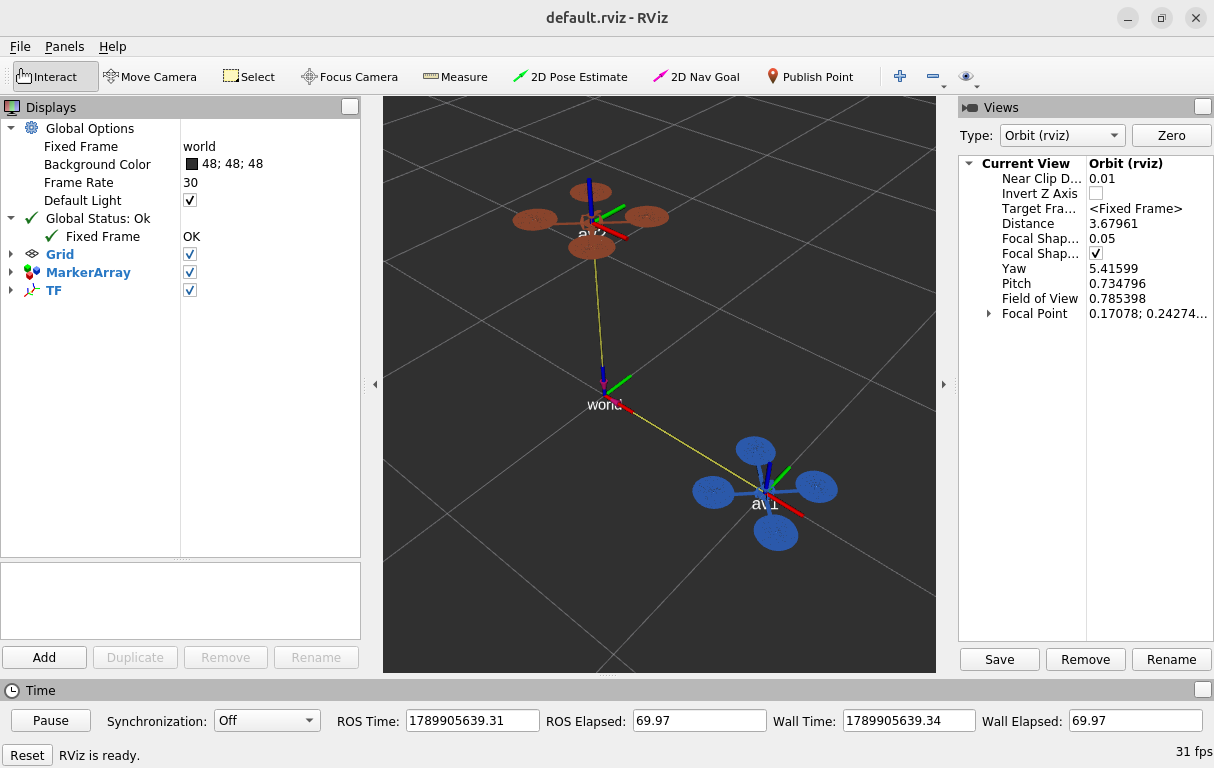
\includegraphics[width=\columnwidth]{static_rviz.png}
\caption{RViz visualization in static mode with both meshes and TF frames.}
\label{fig:static}
\end{figure}

In dynamic mode, Fig.~\ref{fig:world} shows three trajectories. The blue solid curve is AV1's unit circle in the world $x$-$y$ plane. The orange solid curve is AV2's parabola in the world $x$-$z$ plane. The orange dashed curve is the AV2 trajectory expressed in AV1.

\begin{figure}[t]
\centering
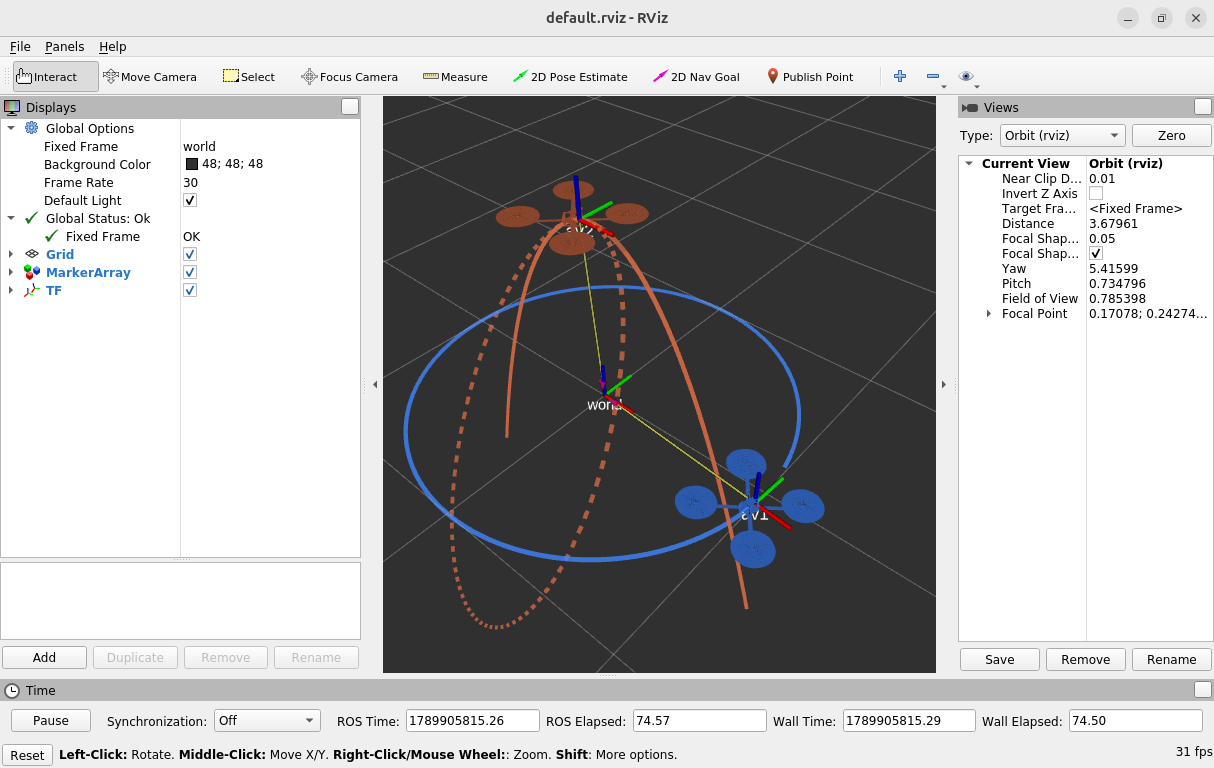
\includegraphics[width=\columnwidth]{dynamic_world_rviz.png}
\caption{Dynamic trajectories visualized in RViz with the fixed frame set to \texttt{world}.}
\label{fig:world}
\end{figure}

Figure~\ref{fig:world_analytic} separates the two world-frame motions into the planes where they are defined. AV1 remains at $z_w=0$ and has a unit-radius circular projection. AV2 remains at $y_w=0$; its horizontal coordinate ranges from $-1$ to $1$, while its height ranges from $-1$ to $1$. The black markers indicate $t=0$. These are analytic plots of Eq.~\eqref{eq:world_positions}, included to make the geometry in the RViz image easier to read.

\begin{figure*}[t]
\centering
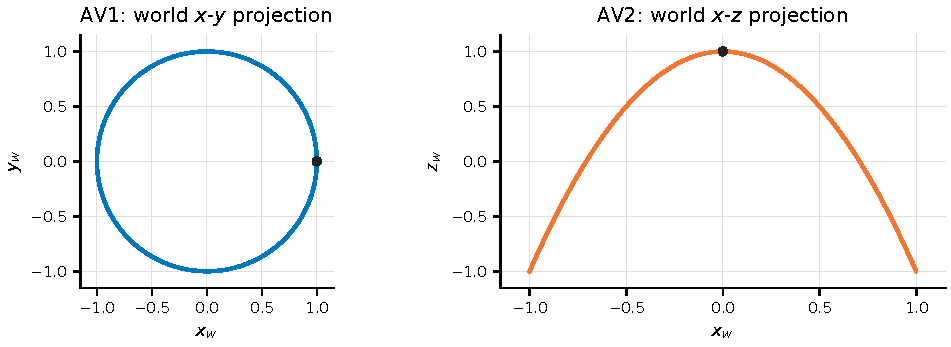
\includegraphics[width=0.82\textwidth]{world_analytic.pdf}
\caption{Analytic world-frame projections over $0\leq t\leq2\pi$. Black markers show the starting positions at $t=0$; the curves are calculated from Eq.~\eqref{eq:world_positions}, not extracted from RViz.}
\label{fig:world_analytic}
\end{figure*}

Changing the RViz fixed frame to \texttt{av1} makes AV1 stationary while the world and AV2 move around it, as shown in Fig.~\ref{fig:av1}. The relative dashed curve forms a closed curve on a slanted plane; its geometry is derived in Section~\ref{sec:math}.

\begin{figure}[t]
\centering
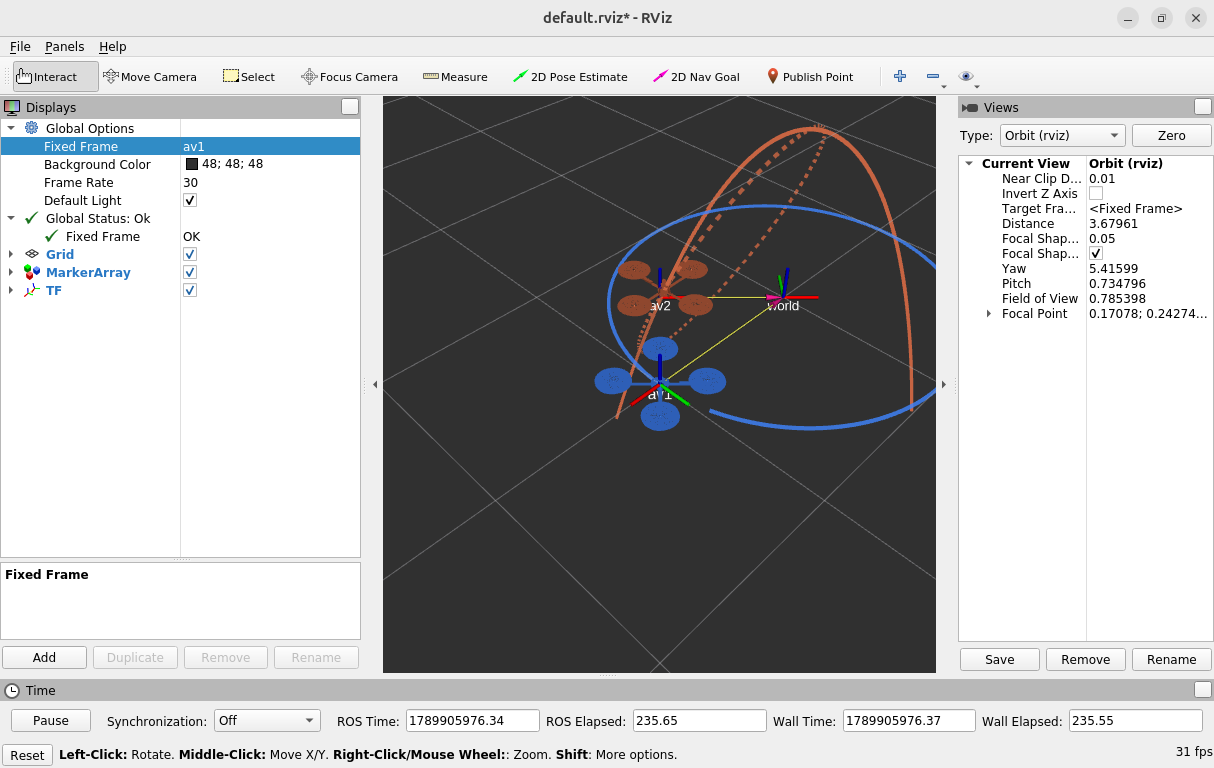
\includegraphics[width=\columnwidth]{dynamic_av1_rviz.png}
\caption{RViz visualization with the fixed frame set to \texttt{av1}.}
\label{fig:av1}
\end{figure}

Table~\ref{tab:plane_check} lists six saved samples obtained from \texttt{tf\_echo av1 av2}: three from an initial capture and three from a second saved log. Their residuals in $z=2y+1$ are at most $0.001$ when computed from the displayed three-decimal coordinates. The table describes the printed TF output rather than a higher-precision estimate of tracking error.

\begin{table}[t]
\caption{Saved AV2 positions in the AV1 frame and plane residuals. The upper and lower groups are from separate TF captures.}
\label{tab:plane_check}
\centering
\small
\begin{tabular}{rrrr}
\toprule
$x$ & $y$ & $z$ & $z-(2y+1)$ \\
\midrule
$-1.149$ & $-0.977$ & $-0.955$ & $-0.001$ \\
$-1.479$ & $-0.356$ & $ 0.288$ & $ 0.000$ \\
$-0.682$ & $-0.114$ & $ 0.771$ & $-0.001$ \\
\midrule
$-1.354$ & $-0.147$ & $ 0.705$ & $-0.001$ \\
$-0.666$ & $-0.128$ & $ 0.743$ & $-0.001$ \\
$-0.801$ & $-0.959$ & $-0.918$ & $ 0.000$ \\
\bottomrule
\end{tabular}
\end{table}

\section{Mathematical Analysis}
\label{sec:math}

\subsection{AV2 world-frame parabola}
From Eq.~\eqref{eq:world_positions}, $x=\sin t$, $y=0$, and
\begin{equation}
z=\cos 2t=1-2\sin^{2}t=1-2x^{2}.
\end{equation}
Thus AV2 lies on the parabola $z=1-2x^{2}$ in the world $x$-$z$ plane.
As $t$ runs from $0$ to $2\pi$, $x=\sin t$ visits both positive and negative halves of this arc and retraces them. The projected parabola alone therefore does not reveal direction of travel or elapsed time; the parametric equations are needed for that information.

\subsection{Position of AV2 relative to AV1}
The inverse of the first transform in Eq.~\eqref{eq:published_transforms} is
\begin{equation}
{}^{1}\mathbf{T}_{w}=
\begin{bmatrix}
\mathbf{R}_{z}(-t)&-\mathbf{R}_{z}(-t){}^{w}\mathbf{o}_{1}\\
\mathbf{0}^{\T}&1
\end{bmatrix}.
\end{equation}
Therefore
\begin{align}
{}^{1}\mathbf{T}_{2}&={}^{1}\mathbf{T}_{w}{}^{w}\mathbf{T}_{2},\\
{}^{1}\mathbf{o}_{2}(t)
&=\mathbf{R}_{z}(-t)
\left({}^{w}\mathbf{o}_{2}-{}^{w}\mathbf{o}_{1}\right)\\
&=\begin{bmatrix}
\sin t\cos t-1\\
-\sin^{2}t\\
\cos 2t
\end{bmatrix}.
\label{eq:relative_position}
\end{align}
The inverse rotation changes both the direction and origin of the coordinate description. Expanding the trigonometric terms makes the relative motion especially simple:
\begin{equation}
{}^{1}\mathbf{o}_{2}(t)=
\begin{bmatrix}
-1+\tfrac12\sin 2t\\
-\tfrac12+\tfrac12\cos 2t\\
\cos 2t
\end{bmatrix}.
\label{eq:relative_harmonic}
\end{equation}
Each component repeats after $\pi$, although the individual world-frame poses repeat after $2\pi$. Figure~\ref{fig:relative_components} shows this relative period over two successive cycles. It also shows that $y$ and $z$ rise and fall together, with $z$ spanning twice the excursion of $y$.

\begin{figure}[t]
\centering
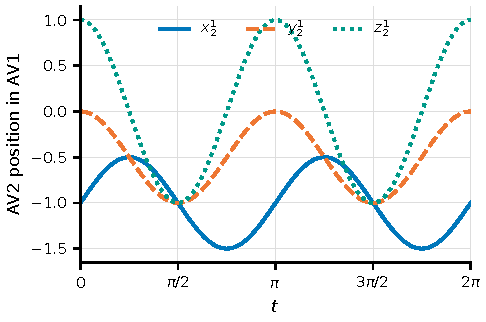
\includegraphics[width=\columnwidth]{relative_components.pdf}
\caption{Analytic components of AV2's position in AV1 from Eq.~\eqref{eq:relative_harmonic}. The interval $0\leq t\leq2\pi$ contains two relative-motion cycles.}
\label{fig:relative_components}
\end{figure}

\subsection{Supporting plane and intrinsic coordinates}
Equation~\eqref{eq:relative_position} gives
\begin{equation}
z=\cos 2t=1-2\sin^{2}t=2y+1,
\end{equation}
so the relative curve lies in
\begin{equation}
\Pi:\quad 2y-z+1=0.
\label{eq:plane}
\end{equation}
The plane normal is proportional to $(0,2,-1)^{\T}$. Since the $x$ component of this normal is zero, the plane contains lines parallel to the AV1 $x$ axis; the linear $y$-$z$ relation sets its tilt.
Choose the plane origin $\mathbf{p}^{1}=(-1,-1/2,0)^{\T}$ and the orthonormal basis
\begin{align}
\mathbf{e}_{x_p}&=\begin{bmatrix}1&0&0\end{bmatrix}^{\T},\nonumber\\
\mathbf{e}_{y_p}&=\frac{1}{\sqrt{5}}
\begin{bmatrix}0&1&2\end{bmatrix}^{\T},\nonumber\\
\mathbf{e}_{z_p}&=\frac{1}{\sqrt{5}}
\begin{bmatrix}0&-2&1\end{bmatrix}^{\T}.
\end{align}
The centered displacement is
\begin{equation}
{}^{1}\mathbf{o}_{2}-\mathbf{p}^{1}=
\begin{bmatrix}
\tfrac12\sin 2t&\tfrac12\cos 2t&\cos 2t
\end{bmatrix}^{\T}.
\end{equation}
Projection onto the plane basis yields
\begin{equation}
x_p=\frac12\sin 2t,\qquad
y_p=\frac{\sqrt{5}}{2}\cos 2t,\qquad z_p=0.
\label{eq:plane_coordinates}
\end{equation}
Eliminating $t$ gives
\begin{equation}
\frac{x_p^2}{(1/2)^2}+\frac{y_p^2}{(\sqrt{5}/2)^2}=1.
\label{eq:ellipse}
\end{equation}
Hence the relative trajectory is an ellipse centered at $\mathbf{p}^{1}$, with semi-axis lengths $1/2$ and $\sqrt{5}/2$.
The longer semi-axis lies along $\mathbf{e}_{y_p}$, a direction tilted in the AV1 $y$-$z$ plane. Figure~\ref{fig:relative_ellipse} plots the ellipse in these intrinsic coordinates and projects the six saved TF positions from Table~\ref{tab:plane_check} onto the same axes. The points fall near the curve at the resolution of the saved coordinates; unlike the continuous black line, they are individual runtime samples.

\begin{figure}[t]
\centering
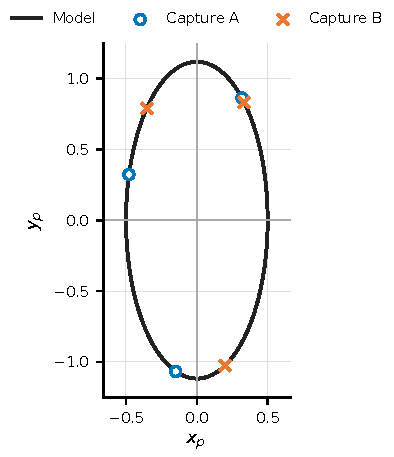
\includegraphics[width=\columnwidth]{relative_ellipse_samples.pdf}
\caption{Analytic relative ellipse and six TF samples in the plane coordinates of Eq.~\eqref{eq:plane_coordinates}. Symbols distinguish the two captures in Table~\ref{tab:plane_check}.}
\label{fig:relative_ellipse}
\end{figure}

\newpage
\balance
\section{Quaternion Operator Properties}
Let $q=[q_1,q_2,q_3,q_4]^{\T}$ use scalar-last convention, and let $\Omega_1(q)$ and $\Omega_2(q)$ denote left- and right-quaternion multiplication as defined in the exercise.

\subsection{Orthogonality}
Direct multiplication gives, for either operator,
\begin{equation}
\Omega_i(q)^{\T}\Omega_i(q)=
\Omega_i(q)\Omega_i(q)^{\T}
=\left(q_1^2+q_2^2+q_3^2+q_4^2\right)\mathbf{I}_4.
\end{equation}
For a unit quaternion the scalar factor is one, so both matrices are orthogonal. The geometric reason is norm multiplicativity:
\begin{equation}
\|q\otimes x\|=\|q\|\,\|x\|=\|x\|,
\end{equation}
and likewise for right multiplication. A linear map preserving every Euclidean norm is orthogonal.

\subsection{Mapping to the identity quaternion}
For unit $q$, orthogonality and the multiplication definition imply
\begin{align}
\Omega_1(q)^{\T}q&=q^{-1}\otimes q=
\begin{bmatrix}0&0&0&1\end{bmatrix}^{\T},\\
\Omega_2(q)^{\T}q&=q\otimes q^{-1}=
\begin{bmatrix}0&0&0&1\end{bmatrix}^{\T}.
\end{align}
Thus both transposed operators map $q$ to the identity rotation quaternion.

\subsection{Commutation of left and right multiplication}
For arbitrary $x,y,z\in\R^4$, quaternion associativity gives
\begin{align}
\Omega_1(x)\Omega_2(y)z
&=x\otimes(z\otimes y)\\
&=(x\otimes z)\otimes y
=\Omega_2(y)\Omega_1(x)z.
\end{align}
Because this holds for every $z$,
\begin{equation}
\Omega_1(x)\Omega_2(y)=\Omega_2(y)\Omega_1(x).
\end{equation}
Furthermore, transposition corresponds to right multiplication by the conjugate: $\Omega_2(y)^{\T}=\Omega_2(y^{*})$. Replacing $y$ by $y^{*}$ in the preceding argument yields
\begin{equation}
\Omega_1(x)\Omega_2(y)^{\T}=\Omega_2(y)^{\T}\Omega_1(x).
\end{equation}

\section{Conclusion}
The ROS implementation produced the prescribed world-frame circle and parabolic arc. Expressing AV2 in AV1 gives a shorter-period relative motion: an ellipse on $2y-z+1=0$ with semi-axes $1/2$ and $\sqrt{5}/2$. The analytic plots clarify the geometry seen in RViz, while the saved TF positions provide discrete samples of the relative path.

\begin{thebibliography}{9}
\bibitem{mitlab}
MIT SPARK Lab, ``VNAV Lab 2: Exercises,'' 2023. [Online]. Available: \url{https://vnav.mit.edu/labs_2023/lab2/exercises.html}

\bibitem{tf2}
Open Robotics, ``tf2: The second generation of the transform library.'' [Online]. Available: \url{https://wiki.ros.org/tf2}
\end{thebibliography}

\end{document}
